\documentclass[14pt,a4paper]{extreport}
\usepackage[top=2cm, left=3cm, bottom=2cm, right=1cm]{geometry}
\usepackage[utf8x]{inputenc} % Включаем поддержку UTF8
\usepackage[russian]{babel} % Пакет поддержки русского языка
\usepackage{lscape}
\usepackage{fancyhdr}
\usepackage{textcase}
\usepackage{graphicx}
\usepackage{caption}
\usepackage{refstyle}


\title{}
\author{}

\begin{document}
%----------ТИТУЛЬНЫЙ-ЛИСТ--------------
	\center
	Министерство образования Республики Беларусь\\
	Учреждение образования «Белорусский государственный университет информатики и радиоэлектроники»
	\vspace*{2cm}
	\endcenter
	\raggedright
	Факультет компьютерных систем и сетей\\
	\medskip
	Кафедра программного обеспечения информационных технологий\\
	\medskip
	Дисциплина:  Компьютерные системы и сети (КСиС)
	\vspace*{2cm}
	\center
	ПОЯСНИТЕЛЬНАЯ ЗАПИСКА\\
	к курсовому проекту\\
	на тему\\
	\medskip
	Веб-сайт доска объявлений\\
	\medskip
	БГУИР КП  1-40 01 0 26 ПЗ
	\vspace*{4cm}
	\endcenter
	\raggedright
	\hspace*{7.94cm}Студент:  гр. 351002 Гучок О.А.\\
	\bigskip
	\hspace*{7.94cm}Руководитель: асс. Третьяков Ф.И.\\
	\center
	\vspace*{2cm}
	Минск 2015
	\pagestyle{empty}
%-------ЛИСТ-ЗАДАНИЯ--------------
	\newpage
	\center
	Учреждение образования\\
	\medskip
	«Белорусский государственный университет информатики и радиоэлектроники»\\
	\medskip
	Факультет компьютерных систем и сетей\\
	\medskip
	\endcenter
	\raggedright
	\hspace*{9.53cm}УТВЕРЖДАЮ\\
	\hspace*{9.53cm}Заведующий кафедрой ПОИТ\\
	\hspace*{9.53cm}\underline{\hspace{6cm}} \\
	\hspace*{11cm}\small (подпись) \normalsize\\
	\hspace*{9.53cm}\underline{\hspace{5cm}}2015 г.\\
	\medskip
	\center
	ЗАДАНИЕ\\
	по курсовому проектированию\\
	\medskip
	\endcenter
	\raggedright
	Студенту \underline{Гучку Олегу Анатольевичу}\\
	\begin{enumerate}
	\item Тема работы \underline{Веб-сайт доска объявлений}\\ 
	\item Срок сдачи студентом законченной работы \underline{DD.MM.YYYY}
	\item Исходные данные к работе \underline{Среда разработки Visual Studio 2013. }
	\item Содержание расчётно-пояснительной записки (перечень вопросов, которые подлежат разработке)\\
	\underline{\hspace*{16cm}}\hspace*{-16cm}Введение. 1. Анализ литературных источников. 2. Постановка задачи\\
	\underline{\hspace*{16cm}}\hspace*{-16cm}3.Разработка программного средства. 4. Руководство по \\
	\underline{\hspace*{16cm}}\hspace*{-16cm}использованию веб-сайта. Заключение. Приложения.
	\item Перечень графического материала (с точным обозначением обязательных чертежей и графиков)\\
	\underline{1. Схема алгоритма}
	\item Консультант по курсовой работе\\
	\underline{Третьяков Ф.И.}  
	\item Дата выдачи задания \underline{DD.MM.YYYY}
	\item Календарный график работы над проектом на весь период проектирования (с обозначением сроков выполнения и процентом от общего объёма работы):\\
	\underline{\hspace*{16cm}}\hspace*{-16cm}раздел 1 к DD.MM.YYYY – 15 \% готовности работы;\\  
	\underline{\hspace*{16cm}}\hspace*{-16cm}разделы 2, 3 к DD.MM.YYYY – 30 \% готовности работы;\\ 
	\underline{\hspace*{16cm}}\hspace*{-16cm}раздел 4 к DD.MM.YYYY – 60 \% готовности работы;\\
	\underline{\hspace*{16cm}}\hspace*{-16cm}раздел 5, 6 к DD.MM.YYYY  –  90 \% готовности работы;\\
	\underline{\hspace*{16cm}}\hspace*{-16cm}оформление пояснительной записки и графического материала к\\
	\underline{\hspace*{16cm}}\hspace*{-16cm}DD.MM.YYYY – 100 \% готовности работы.\\
	\underline{\hspace*{16cm}}\hspace*{-16cm}Защита курсового проекта с DD по DD декабря YYYY г.\\
	\end{enumerate}
	\hspace*{7cm}РУКОВОДИТЕЛЬ\underline{\hspace*{6cm}}\hspace*{-3.9cm}Третьяков Ф.И.\\
	\hspace*{11.5cm}\small (подпись) \normalsize\\
	\bigskip
	Задание принял к исполнению \underline{\hspace*{10.5cm}}\hspace*{-8cm}Гучок О.А. DD.MM.YYYYг.\\
	\hspace*{7cm}\small (дата и подпись студента) \normalsize\\
	%-------СОДЕРЖАНИЕ--------------
	\newpage
	\pagestyle{plain}
	%\renewcommand{\headrulewidth}{0px}
	%\fancypagestyle{plain}{\cfoot{}\rfoot{\thepage}}
	
	\renewcommand\contentsname{\center\normalsize \textbf{СОДЕРЖАНИЕ} \endcenter}
	\tableofcontents
	\endcenter
	%-----ВВЕДЕНИЕ-----
	\newpage
	\addcontentsline{toc}{section}{ВВЕДЕНИЕ}
	\section*{\center\normalsize ВВЕДЕНИЕ \endcenter}
	\hspace{4ex}
	
	\parindent = 1cmИнтернет впервые был создан в 60-х гг. прошлого века как проект Министерства обороны США. Он получил название ARPANET (Advanced Research Projects Agency Network — сеть Агентства по перспективным исследовательским проектам). Его основной целью было объединение различных компьютеров, разбросанных по Западному побережью США с тем, чтобы они могли взаимодействовать друг с другом даже в случае начала атомной войны. В то время компьютеры были очень редкими и дорогостоящими устройствами, которые могли позволить себе только университеты и правительственные организации. Связав воедино несколько компьютеров, можно было организовать общий доступ к различной информации и данным, что еще больше увеличивало ценность каждого отдельного компьютера. Протокол, предназначенный для работы в данной сети, был разработан таким образом, чтобы быть устойчивым к нарушениям целостности сети. Это было сделано для того, чтобы даже при выходе из строя в результате ядерной атаки одного или нескольких компьютеров, сеть сохраняла бы свою работоспособность.\par
	Результатом разработки ARPANET явилось создание TCP/IP (Transmission Control Protocol/Internet Protocol — протокол управления передачей/межсетевой протокол). Это протокол, позволяющий вести обмен сигналами, в которых содержатся компьютерные данные и информация, по телефонным линиям, по волоконно-оптическим кабелям и через спутники. Протокол TCP/IP позволяет различным компьютерам обмениваться между собой информацией по сети, и его принятие расчистило дорогу для появления Интернета в том виде, в котором он знаком нам сегодня.\par
	Бесчисленное множество новых технологий, вызванных бурным ростом информатизации общества, делает нашу жизнь невозможной без быстрого доступа к информации. В наше время очень легко получить информацию, одним из способов быстрого доступа к ней является сайт.\par
	Создание сайтов на сегодняшний день, становится одной из наиболее актуальных и востребованных услуг. Именно поэтому, большинство компаний уже оценили все преимущества такого предложения как создание сайтов и позаботились о разработке подходящего ресурса.\par
	Пользователю приятно посещать те Web-страницы, которые имеют стильное оформление, не отягощены чрезмерно графикой и анимацией, быстро загружаются и правильно отображаются в окне Web-браузера. Но может возникнуть и другая проблема - сайт может оказаться не интересным пользователю и та информация, которую он несет, окажется не востребованной. Именно поэтому важно, чтобы сайт отвечал всем требованиям пользователя.\par
	Актуальность данной работы заключается в том, что с учетом скорости развития сети Интернет и направления e-commerce, рынок WEB-разработки огромен и очень перспективен.\par
	Целью работы является формирование теоретических знаний по проектированию web-сайта и практических навыков по его разработке. Выбранная технология - ASP.NET MVC.\par
	Инфраструктура ASP.NET MVC Framework реализует шаблон MVC и при этом обеспечивает существенно улучшенное разделение ответственности. На самом деле в ASP.NET MVC внедрен современный вариант MVC, который особенно хорошо подходит для веб-приложений.\par
	За счет принятия и адаптации шаблона MVC инфраструктура ASP.NET MVC Framework составляет сильную конкуренцию Ruby on Rails и аналогичным платформам, выводя модель MVC в авангард развития мира .NET. Обобщая опыт и наиболее рекомендуемые приемы, обнаруженные разработчиками, которые используют другие платформы, ASP.NET MVC во многих отношениях превзошла даже то, что может предложить Rails.\par	

	%-----АНАЛИЗ ЛИТЕРАТУРНЫХ ИСТОЧНИКОВ----
	\newpage
	\addcontentsline{toc}{section}{1 АНАЛИЗ ЛИТЕРАТУРНЫХ ИСТОЧНИКОВ}
	\addcontentsline{toc}{subsection}{1.1 Технологии создания web-страниц}
	\addcontentsline{toc}{subsection}{1.2 Появление ASP.NET MVC}
	\addcontentsline{toc}{subsection}{1.3 Паттерн MVC}
	\addcontentsline{toc}{subsection}{1.4 Преимущества ASP.NET MVC}
	\section*{\normalsize\hspace{4ex}1 АНАЛИЗ ЛИТЕРАТУРНЫХ ИСТОЧНИКОВ}
	\textbf{1.1  Технологии создания web-страниц}

	\parindent=1cm Итак, Интернет — это цельная связанная сеть компьютеров, которая охватывает весь земной шар. На миллионах серверов располагаются миллиарды web-страниц, групп электронной почты, дискуссионных страниц и FTP-сайтов. Интернет целиком работает в режиме онлайн, включая электронную почту, FTP, новости, Gophet-сайты, чат-программы и т. п. World Wide Web появилась позже Интернета. Первый web-сервер заработал в 1991 г., но на сегодняшний день Всемирная паутина — это огромная часть Интернета, состоящая из взаимосвязанных web-страниц, в которых содержится текст, графика и мультипликация. Ключевым компонентом World Wide Web являются гиперссылки (текстовые или графические), которые позволяют пользователю переходить на другие web-страницы. Это оказывается возможным благодаря использованию HyperText Markup Language (HTML, язык гипертекстовой разметки).\par
	Интернет представляет собой клиент-серверную систему. Т.е. вся информация хранится на серверах, которые по мере надобности посылают информацию клиентам. Сервер — это приложение, выполняющееся на некотором компьютере и обеспечивающее доступ к информации, файлам или данным, которые запрашиваются каким-либо другим лицом, приложением или компьютером. Местоположение серверов определяется с помощью Uniform Resource Locator (URL — универсальный указатель ресурса). Это особый адрес web-страницы, по которому она располагается в World Wide Web.\par 		Клиентом называется особая часть программного обеспечения, выполняющаяся на компьютере. Наиболее распространенным клиентом в Интернете является браузер — специальная программа, позволяющая пользователю вводить адреса или использовать гиперссылки на web - страницах для поиска новых web-страниц. Она управляет отправкой запросов web-серверу и выводом на экран полученной от web-сервера web-страницы.\par
	Вся работа по отправеке и получению web-страниц ведется через протокол HTTP (Hypertext Transfer Protocol). Это прикладной протокол, позволяющий браузерам и серверам взаимодействовать друг с другом и обмениваться между собой данными.\par
	Использование одного лишь HTML невозможно в наше время. Во-первых это связано с созданием web-страниц: очень сложно обновлять страницы вручную. Во-вторых, в чистом HTML отсутствует какая-либо интерактивность и возможность сзаимодействовать на с серверами на пользовательском уровне. Например, не было бы почтовых служб, чатов и форумов. Проще говоря, это означало бы полную статичность.\par
	Чтобы «оживить» Web, т.е. перейти от структурного предъявления гипертекстовой информации к событийному был разработан DHTML (Dynamic HyperText Markup Language). Основной отличительной особенностью DHTML от HTML является возможность взаимодействия DHTML-документов с пользователем на клиентском компьютере, что в значительной степени обогащает возможности создаваемых с их помощью Web-страниц и Web-приложений и в то же время сводит часть взаимодействия пользователя с сервером к взаимодействию пользователя с DHTML-документом.
	Динамичность осуществляется при помощи языков сценариев, таких как JavaScript и VBScript. Но эта динамичность присуща только для клиентской части, взаимодействие с сервером все так же остается на примитивном уровне и позволяет отправлять всем пользователям только одну и ту же статическую информацию.\par 
	Поэтому был разработан Common Gateway Interface (CGI — интерфейс общего шлюза), который позволял web-страницам вызывать приложения, расположенные на web-серверах. Такие приложения могли создаваться на произвольном языке программирования, но чаще всего они писались на C/C++ или на Perl. Но CGI требовало огромных ресурсов,- для каждого подключившегося к серверу пользователя запускался свой экземпляр CGI, ни один популярный сервер не смог бы работать в нормальном режиме.\par
	В итоге было создано большое количество различных инструментов и языков программирования, которые позволяют создавать активные web-страницы. Вот некоторые из этих технологий:\par
	• Active Server Pages\par
	• PHP\par
	• ColdFusion\par
	• WebSphere\par
	• Java Server Pages\par	
	Несмотря на то, что PHP является лидером этой сферы деятельности, ASP даёт программистам большую свободу и простоту. Главным недостатком является цена и производительность Windows серверов.\par
	~\\

	\textbf{1.2 Появление ASP.NET MVC}

	\parindent=1cm ASP.NET MVC - это инфраструктура для разработки веб-приложений от Microsoft, которая сочетает в себе эффективность и аккуратность архитектуры "модель-представление-контроллер" (model-view-controller - MVC), новейшие идеи и приемы гибкой разработки, а также все лучшее из существующей платформы ASP.NET. Она представляет собой полномасштабную альтернативу традиционной технологии ASP.NET Web Forms, предоставляя преимущества для всех проектов веб-разработки, кроме самых тривиальных.\par
	Важно различать архитектурный шаблон MVC и инфраструктуру ASP.NET MVC Framework. Шаблон MVC далеко не нов (его появление датируется 1978 г. и связано с проектом Smalltalk в Xerox PARC), но в наши дни он завоевал огромную популярность в качестве шаблона для веб-приложений по перечисленным ниже причинам:\par
	• Взаимодействие пользователя с приложением MVC осуществляется в соответствии с естественным циклом: пользователь предпринимает действие, в ответ на которое приложение изменяет свою модель данных и доставляет обновленное представление пользователю. Затем цикл повторяется. Это хорошо укладывается в схему веб-приложений, предоставляемых в виде последовательностей запросов и ответов HTTP.\par
	• Веб-приложения, нуждающиеся в комбинировании нескольких технологий (например, баз данных, HTML-разметки и исполняемого кода), обычно разделяются на ряд слоев или уровней. Полученные в результате шаблоны естественным образом вписываются в концепции MVC.\par
	~\\

	\textbf{1.3 Паттерн MVC}

	\parindent=1cm Шаблон MVC, лежащий в основе новой платформы, подразумевает взаимодействие трех компонентов: контроллера (controller), модели (model) и представления (view)(Рис. 1).\par
	Контроллер (controller) представляет класс, с которого собственно и начинается работа приложения. Этот класс обеспечивает связь между моделью и представлением. Получая вводимые пользователем данные, контроллер исходя из внутренней логики при необходимости обращается к модели и генерирует соответствующее представление.\par
	Представление (view) - это собственно визуальная часть или пользовательский интерфейс приложения - например, html-страница, через которую пользователь, зашедший на сайт, взаимодействует с веб-приложением.\par
	Модель (model) представляет набор классов, описывающих логику используемых данных.\par
	\begin{figure}[h]
	\begin{center}
	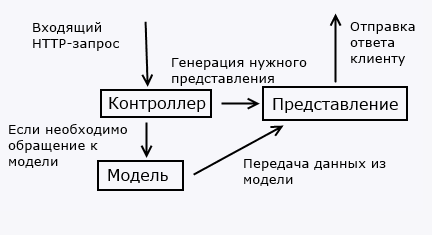
\includegraphics[scale=0.9]{mvc}
	\caption{ Схема паттерна MVC}
	\end{center}
	\end{figure}
	~\\

	\textbf{1.4 Преимущества ASP.NET MVC}
	
	\parindent=1cm ASP.NET MVC имеет следующие преимущества:\par
	• Разделение ответственности. В MVC приложение состоит из трех частей: контроллера, представления и модели, каждая из которых выполняет свои специфичные функции. В итоге приложение будет легче поддерживать модифицировать в будущем.\par
	• В силу разделения ответственности приложения mvc обладают лучшей тестируемостью. И мы можем тестировать отдельные компоненты независимо друг от друга.\par
	• Соответствие протоколу HTTP. Приложения MVC в отличие от веб-форм не поддерживают объекты состояния (ViewState). Ясность и простота платформы позволяют добиться большего контроля над работой приложения.\par
	• Гибкость. Вы можете настраивать различные компоненты платформы по своему усмотрению. Изменять какие-либо части конвейера работы MVC или адаптировать его к своим нуждам и потребностям.\par
	• Инфраструктура ASP.NET MVC имеет открытый код. В отличие от предшествующих платформ веб-разработки производства Microsoft, первоначальный исходный код ASP.NET MVC доступен для свободной загрузки и даже для модификации и компиляции с целью получения собственной версии этой инфраструктуры. Это буквально неоценимо при отладке кода, обращающегося к системному компоненту, когда требуется пошагово выполнить его код (и даже ознакомиться с комментариями программистов, написавших этот код). Это также полезно, если вы создаете усовершенствованный компонент и хотите видеть, какие существуют возможности разработки, или узнать, как действительно работают встроенные компоненты.\par

	%-----ПОСТАНОВКА ЗАДАЧИ-----f
	\newpage
	\addcontentsline{toc}{section}{2 ПОСТАНОВКА ЗАДАЧИ}
	\section*{\normalsize\hspace{2ex}2 ПОСТАНОВКА ЗАДАЧИ}

	%-----РАЗРАБОТКА ИГРОВОГО ПРИЛОЖЕНИЯ----
	\newpage
	\addcontentsline{toc}{section}{3 РАЗРАБОТКА ПРИЛОЖЕНИЯ}
	\section*{\normalsize\hspace{4ex}3 РАЗРАБОТКА ПРИЛОЖЕНИЯ}

	%-----РУКОВОДСТВО ПО УСТАНОВКЕ И ИСПОЛЬЗОВАНИЮ ИГРОВОГО ПРИЛОЖЕНИЯ------
	\newpage
	\addcontentsline{toc}{section}{4 РУКОВОДСТВО ПО УСТАНОВКЕ И ИСПОЛЬЗОВАНИЮ ВЕБ-САЙТА}
	\section*{\normalsize\hspace{4ex}4 РУКОВОДСТВО ПО УСТАНОВКЕ И ИСПОЛЬЗОВАНИЮ ВЕБ-САЙТА}
	\hspace{4ex}ИСПОЛЬЗОВАНИЕ
	%-------ЗАКЛЮЧЕНИЕ-------
	\newpage
	\addcontentsline{toc}{section}{ЗАКЛЮЧЕНИЕ}
	\section*{\center\normalsize ЗАКЛЮЧЕНИЕ \endcenter}
	\hspace{4ex}Что получилось в результате выполнения курсовой работы, что планируется добавить в будущем.
	%----СПИСОК ИСПОЛЬЗОВАННОЙ ЛИТЕРАТУРЫ-------
	\newpage
	\addcontentsline{toc}{section}{СПИСОК ИСПОЛЬЗОВАННОЙ ЛИТЕРАТУРЫ}
	\section*{\center\normalsize СПИСОК ИСПОЛЬЗОВАННОЙ ЛИТЕРАТУРЫ \endcenter}
	%----ПРИЛОЖЕНИЕ А (обязательное) Исходный код программы----
	\begin{landscape}
	\newpage
	\addcontentsline{toc}{section}{ПРИЛОЖЕНИЕ А}
	\section*{\center\normalsize ПРИЛОЖЕНИЕ А\\(обязательное)\\Исходный код программы \endcenter}
	<html>HTML-код</html>
	\end{landscape}
	
	
\end{document}          
